\begin{figure}[htb]
\centering
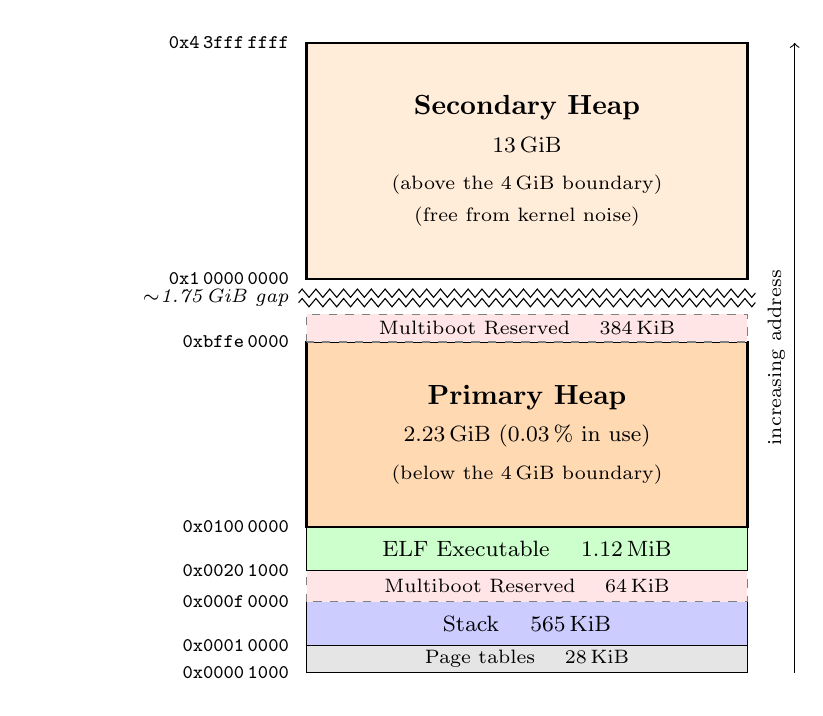
\begin{tikzpicture}[
  every node/.style={font=\footnotesize},
  addr/.style={anchor=east, font=\ttfamily\scriptsize,
               text width=3.2cm, align=right},
]

%% --- Zone 1: low addresses ---

\draw[fill=gray!20]  (0,0.00) rectangle (5.6,0.35);
\node[font=\scriptsize] at (2.8,0.175) {Page tables \quad 28\,KiB};
\node[addr] at (-0.1,0.00) {0x0000\,1000};

\draw[fill=blue!20]  (0,0.35) rectangle (5.6,0.90);
\node at (2.8,0.625) {Stack \quad 565\,KiB};
\node[addr] at (-0.1,0.35) {0x0001\,0000};

\draw[fill=red!10, draw=gray, dashed] (0,0.90) rectangle (5.6,1.30);
\node[font=\scriptsize] at (2.8,1.10) {Multiboot Reserved \quad 64\,KiB};
\node[addr] at (-0.1,0.90) {0x000f\,0000};

\draw[fill=green!20] (0,1.30) rectangle (5.6,1.85);
\node at (2.8,1.575) {ELF Executable \quad 1.12\,MiB};
\node[addr] at (-0.1,1.30) {0x0020\,1000};

%% --- Zone 2: primary heap (below 4 GiB) ---
\draw[fill=orange!30, thick] (0,1.85) rectangle (5.6,4.20);
\node[align=center] at (2.8,3.025)
  {\normalsize\textbf{Primary Heap}\\[4pt]
   2.23\,GiB (0.03\,\% in use)\\[4pt]
   \scriptsize (below the 4\,GiB boundary)};
\node[addr] at (-0.1,1.85) {0x0100\,0000};

\draw[fill=red!10, draw=gray, dashed] (0,4.20) rectangle (5.6,4.55);
\node[font=\scriptsize] at (2.8,4.375) {Multiboot Reserved \quad 384\,KiB};
\node[addr] at (-0.1,4.20) {0xbffe\,0000};

%% --- Axis break: small gap up to the 4 GiB boundary ---
\foreach \yy in {4.70,4.82} {
  \draw[decorate,decoration={zigzag,amplitude=1.5pt,segment length=5pt}]
    (-0.1,\yy) -- (5.7,\yy);
}
\node[anchor=east, font=\scriptsize\itshape] at (-0.1,4.76) {$\sim$1.75\,GiB gap};

%% --- Zone 3: secondary heap (above 4 GiB) ---
\draw[fill=orange!15, thick] (0,5.00) rectangle (5.6,8.00);
\node[align=center] at (2.8,6.50)
  {\normalsize\textbf{Secondary Heap}\\[4pt]
   13\,GiB\\[4pt]
   \scriptsize (above the 4\,GiB boundary)\\[2pt]
   \scriptsize (free from kernel noise)};
\node[addr] at (-0.1,5.00) {0x1\,0000\,0000};
\node[addr] at (-0.1,8.00) {0x4\,3fff\,ffff};

%% --- Increasing-address arrow ---
\draw[->] (6.2,0.00) -- (6.2,8.00)
  node[midway, rotate=90, anchor=south, font=\scriptsize] {increasing address};

\end{tikzpicture}
\caption{Physical memory of a 16\,GiB IncludeOS guest after this work,
  split into two heaps at the 4\,GiB boundary (not to scale; the zigzag
  marks a gap left out). The primary heap, below 4\,GiB, holds everything
  the kernel allocates during boot, and is the one 32-bit DMA devices can
  reach. The secondary heap, above 4\,GiB, is almost six times larger and
  untouched when the application starts.}
\label{fig:heap-regions}
\end{figure}
